\chapter{Partially Reconstructed Backgrounds}
\label{chap:apdx_partbkg}
Decays where at least one particle is lost during reconstruction are called \textit{partially reconstructed} decays.
In the following we discuss decays akin to \decay{\Lb}{\Dstarz\Lz} with \decay{\Dstarz}{\Dz\PX} where the \PX is lost during reconstruction.
In particular, this description is applicable for the decays \decay{\Lb/\Xibz}{\Dstarz\Lz} with \decay{\Dstarz}{\Dz\piz} and \decay{\Dstarz}{\Dz\Pgamma}, as well as \decay{\Lb/\Xibz}{\Dz\Sz} with \decay{\Sz}{\Lz\Pgamma}, and \decay{\Xibz}{\Dz\Xiz} with \decay{\Xiz}{\Lz\piz} which are considered as critical (partially reconstructed) background events in the invariant mass distribution of \decay{\Lb/\Xibz}{\Dz\Lz} events.
\begin{figure}[htbp]
    \centering
    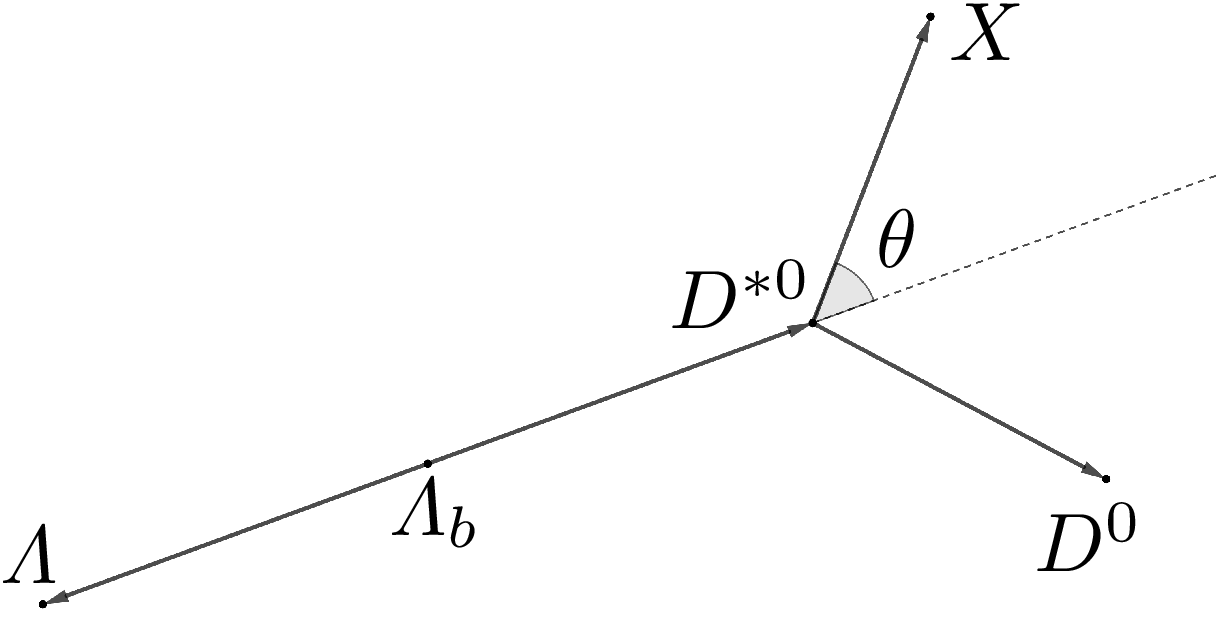
\includegraphics[scale=1.]{misc/decay_Lb2DstarLz.png}
    \caption{Decay topology of \decay{\Lb}{\Dstarz\Lz} with \decay{\Dstarz}{\Dz\PX} in the \Lb rest frame.}
    \label{fig:apdx_partbkg_decay}
\end{figure}
In the following we briefly introduce the notation and then find a explicit solution for the contribution of the various partially reconstructed backgrounds to the invariant mass $m(\Dz\Lz)$ as a function of the opening angle $\theta$ (\cf{}~Fig.~\ref{fig:apdx_partbkg_decay}).
We then discuss the implications of polarization effects and establish a universal fit model.

\section{Kinematics of Partially Reconstructed Decays}
The invariant mass is a Lorentz scalar and can thus be calculated in any frame of reference.
For the sake of simplicity, we choose the CMS of the \Lb particle and determine the spurious, reconstructed invariant mass of the \Lb, denoted as $M$, here, without contributions from the left out particle \PX as
\begin{equation}
    \label{eq:apdx_partbkg_M}
    M = \sqrt{\left(E_{\Lz} + E_{\PD} \right)^2 - \left(p - p_{\parallel,\PD} \right)^2 - \left(p_{T,\PD}\right)^2} \,,
\end{equation}
where $E_{\Lz}$ and $E_{\PD}$ are the energies of the \Lz and \Dz, $p$ is the momentum of the \Lb and \Dstarz, and $p_{\parallel,\PD}$ and $p_{T,\PD}$ are the parallel and transversal components of the \Dz momentum vector w.r.t.\ the flight direction of the \Dstarz particle, respectively.

The energy of the \Lz particle is given by its invariant mass $m_{\Lz}$ and its momentum $p$
\begin{equation*}
    E_{\Lz} = \sqrt{m_{\Lz}^2 + p^2} \,,
\end{equation*}
where $p$ is given by the invariant masses of the \Lb, \Dstarz and \Lz particle
\begin{equation*}
    p = \frac{\sqrt{ \left(m_{\Lb}^2 - \left(m_{\Dstar} + m_{\Lz} \right)^2 \right) \left( m_{\Lb}^2 - \left(m_{\Dstar} - m_{\Lb} \right)^2 \right) }}{2 m_{\Lb}^2} \,.
\end{equation*}
The energy and momentum of the \Dz particle is found by boosting the corresponding energy $E'_{\PD}$ from the CMS of its mother \Dstarz into the CMS of the \Lb:
\begin{align*}
    E_{\PD} &= \gamma \sqrt{m_{\PD}^2 + p^2} + \sqrt{\gamma^2 - 1} \, p' \cos \theta \,, \\
    p_{\parallel,\PD} &= \sqrt{\left( \gamma^2 - 1 \right) \left(m_{\PD}^2 + p'^2 \right)} + \gamma \, p' \cos \theta \,, \\
    p_{T,\PD} &= p'_{T,\PD} = p' \sin \theta \,,
\end{align*}
where we defined the angle $\theta$ as shown in Fig.~\ref{fig:apdx_partbkg_decay}.
The variable $p'$ is the momentum of the \Dz and \PX particle in the CMS of the \Dstarz particle and is given by the invariant masses of \Dstarz, \Dz and \Px particle 
\begin{equation*}
    p' = \frac{\sqrt{ \left(m_{\Dstar}^2 - \left(m_{\PD} + m_{\PX} \right)^2 \right) \left( m_{\Dstar}^2 - \left(m_{\PD} - m_{\PX} \right)^2 \right) }}{2 m_{\Dstar}^2} \,,
\end{equation*}
whereas the Lorentz factor $\gamma$ is given by the kinematics of the \Dstarz in the \Lb CMS
\begin{equation*}
    \gamma = \frac{E_{\Dstar}}{m_{\Dstar}} = \frac{\sqrt{m^2_{\Dstar} + p^2}}{m_{\Dstar}} = \sqrt{1 + \left( \frac{p}{m_{\Dstar}} \right)^2} \,.
\end{equation*}
Insertion into Eq.~\eqref{eq:apdx_partbkg_M} yields
\begin{align*}
    M^2\;=\;\;& \left( \sqrt{m_{\Lz}^2 + p^2} + \gamma \sqrt{m_{\PD}^2 + \left(p' \right)^2} + \sqrt{\gamma^2 - 1} p' \cos \theta \right)^2 \\
    &\quad\quad - \left( p - \sqrt{\left( \gamma^2 - 1 \right) \left(m_{\PD}^2 + \left(p' \right)^2 \right)} - \gamma p' \cos \theta \right)^2 - \left(p' \sin \theta \right)^2 \\
    =\;\;& 2 \left[ \left( \sqrt{m_{\Lz}^2 + p^2} + \gamma \sqrt{m_{\PD}^2 + \left(p' \right)^2} \right) \sqrt{\gamma^2 - 1} \right. \\
    &\quad\quad + \left. \left( p - \sqrt{\left( \gamma^2 - 1 \right) \left(m_{\PD}^2 + \left(p' \right)^2 \right)} \right) \gamma \right] p' \cos \theta \\
    &\quad\quad + \left( \sqrt{m_{\Lz}^2 + p^2} + \gamma \sqrt{m_{\PD}^2 + \left(p' \right)^2} \right)^2 - \left( p - \sqrt{\left( \gamma^2 - 1 \right) \left(m_{\PD}^2 + \left(p' \right)^2 \right)} \right)^2 - \left(p' \right)^2 \\
    =\;\;& 2 \left[ \sqrt{\left(\gamma^2 - 1 \right) \left( m_{\Lz}^2 + p^2 \right)} + p \gamma \right] p' \cos \theta \\
    &\quad\quad + m_{\Lz}^2 + m_{\PD}^2 + 2 \sqrt{m_{\PD}^2 + \left(p' \right)^2} \left( \gamma \sqrt{m_{\Lz}^2 + p^2} + p \sqrt{ \gamma^2 - 1} \right) \\
    =\;\;& 2 \, \frac{m_{\Lb}}{m_{\Dstar}} \, p p' \cos \theta + m_{\Lz}^2 + m_{\PD}^2 + \left( m_{\Lb}^2 - m_{\Lz}^2 - m_{\Dstar}^2 \right) \sqrt{\frac{m_{\PD}^2 + \left(p' \right)^2}{m_{\Dstar}^2}} \,.
\end{align*}
In the case of \decay{\Dstarz}{\Dz\Pgamma} the expression can be simplified further by using $m_{\PX} = 0$:
\begin{multline*}
    \left( M(\theta) \right)^2 = \sqrt{\left( m_{\Lb}^2 - (m_{\Lz} + m_{\Dstar})^2 \right) \left( m_{\Lb}^2 - (m_{\Lz} - m_{\Dstar})^2 \right)} \times \frac{m_{\Dstar}^2 - m_{\PD}^2}{2 m_{\Lb} m_{\Dstar}^3} \cos \theta \\
    \times \frac{m_{\Lb}^2 (m_{\Dstar}^2 + m_{\PD}^2) + (m_{\Lz}^2 - m_{\Dstar}^2)(m_{\Dstar}^2 - m_{\PD}^2)}{2 m_{\Dstar}^2} \,.
\end{multline*}
The spurious, reconstructed invariant mass $m(\Lb) = M(\theta)$ is thus distributed as
\begin{equation*}
    \label{eq:apdx_partbkg_mtheta}
    M(\theta) = \sqrt{a^2 + b^2 \cos(\theta)} \,,
\end{equation*}
with positive constants $a$ and $b$ that are a given by the invariant masses of the decaying daughter and grand-daughter particles.
The kinematic boundaries are given by $M(0)$ and $M(\pi)$.
In Tab.~\ref{tab:apdx_partbkg_boundaries} we list the kinematic boundaries for \decay{\Lb/\Xibz}{\Dstarz\Lz} with \decay{\Dstarz}{\Dz\piz} and \decay{\Dstarz}{\Dz\Pgamma}, as well as \decay{\Lb/\Xibz}{\Dz\Sz} with \decay{\Sz}{\Lz\Pgamma}, and \decay{\Xibz}{\Dz\Xiz} with \decay{\Xiz}{\Lz\piz}.
\begin{table}[htbp]
    \centering
    \caption{Kinematic boundaries of the invariant mass $m(\Dz\Lz)$, as well as parameters $a$ and $b$ (\cf{}~Eq.~\eqref{eq:apdx_partbkg_mtheta}) for various \Lb and \Xibz decays.}
    \label{tab:apdx_partbkg_boundaries}
    \begin{tabular}{l%
                    S[separate-uncertainty=false,table-format=4.6]%
                    S[separate-uncertainty=false,table-format=4.6]%
                    S[separate-uncertainty=false,table-format=4.6]%
                    S[separate-uncertainty=false,table-format=4.6]}
        \toprule
        Decay channel & {min [\mevcc]} & {max [\mevcc]} & {$a$ [\mevcc]} & {$b$ \mevcc} \\
        \midrule
        %\decay{\Lb}{\Dstar\Lz}, \decay{\Dstar}{\PD\pion} & 5354.1 \pm 0.4 & 5448.19 \pm 0.21 & 5401.36 \pm 0.19 & 712.8 \pm 1.8 \\
        %\decay{\Lb}{\Dstar\Lz}, \decay{\Dstar}{\PD\Pgamma} & 5253.19 \pm 0.23 & 5556.29 \pm 0.18 & 5406.87 \pm 0.19 & 1279.92 \pm 0.27 \\
        %\decay{\Lb}{\PD\Sigmares}, \decay{\Sigmares}{\Lz\Pgamma} & 5309.37 \pm 0.18 & 5593.12 \pm 0.17 & 5453.09 \pm 0.17 & 1243.72 \pm 0.17 \\
        %\decay{\Xib}{\Dstar\Lz}, \decay{\Dstar}{\PD\pion} & 5518.6 \pm 0.6 & 5616.9 \pm 0.5 & 5568.0 \pm 0.5 & 739.8 \pm 1.9 \\
        %\decay{\Xib}{\Dstar\Lz}, \decay{\Dstar}{\PD\Pgamma} & 5413.1 \pm 0.5 & 5729.8 \pm 0.5 & 5573.7 \pm 0.5 & 1328.47 \pm 0.31 \\
        %\decay{\Xib}{\PD\Sigmares}, \decay{\Sigmares}{\Lz\Pgamma} & 5469.6 \pm 0.5 & 5765.7 \pm 0.5 & 5619.6 \pm 0.5 & 1289.79 \pm 0.22 \\
        %\decay{\Xib}{\PD\Xires}, \decay{\Xires}{\Lz\pion} & 5145.0 \pm 0.8 & 5605.3 \pm 0.5 & 5380.0 \pm 0.6 & 1573.0 \pm 1.2 \\
        \decay{\Lb}{\Dstar\Lz}, \decay{\Dstar}{\PD\pion} & 5350.2 \pm 0.4 & 5452.06 \pm 0.23 & 5401.36 \pm 0.19 & 741.8 \pm 1.9 \\
        \decay{\Lb}{\Dstar\Lz}, \decay{\Dstar}{\PD\Pgamma} & 5240.66 \pm 0.24 & 5568.11 \pm 0.17 & 5406.87 \pm 0.19 & 1330.28 \pm 0.31 \\
        \decay{\Lb}{\PD\Sigmares}, \decay{\Sigmares}{\Lz\Pgamma} & 5300.33 \pm 0.18 & 5601.69 \pm 0.17 & 5453.09 \pm 0.17 & 1281.69 \pm 0.19 \\
        \decay{\Xib}{\Dstar\Lz}, \decay{\Dstar}{\PD\pion} & 5514.5 \pm 0.6 & 5620.9 \pm 0.5 & 5568.0 \pm 0.5 & 769.8 \pm 2.0 \\
        \decay{\Xib}{\Dstar\Lz}, \decay{\Dstar}{\PD\Pgamma} & 5400.0 \pm 0.5 & 5742.1 \pm 0.5 & 5573.7 \pm 0.5 & 1380.48 \pm 0.35 \\
        \decay{\Xib}{\PD\Sigmares}, \decay{\Sigmares}{\Lz\Pgamma} & 5460.1 \pm 0.5 & 5774.7 \pm 0.5 & 5619.6 \pm 0.5 & 1329.34 \pm 0.24 \\
        \decay{\Xib}{\PD\Xires}, \decay{\Xires}{\Lz\pion} & 5106.4 \pm 0.9 & 5640.4 \pm 0.5 & 5380.0 \pm 0.6 & 1693.9 \pm 1.4 \\
        \bottomrule
    \end{tabular}
\end{table}

\section{Implication of Polarization}
In general, $\cos \theta$ in Eq.~\eqref{eq:apdx_partbkg_mtheta} will not be distributed uniformly for \Lb / \Xibz decays, even for unpolarized \Lb / \Xibz particles, since all involved particles in the respective decay chain carry non-zero spin themselves and therefore will be polarized.
These polarizations are distributed by the weak interaction in a non-trivial manner.
For a given distribution of $f(\cos \theta)$ in the \Lb rest frame, the function $M(\cos \theta) = \sqrt{a^2 + b^2 \cos \theta}$ is distributed according to 
\begin{equation*}
    g(m) = \frac{f \! \left(M^{-1}(m) \right)}{M' \! \left(M^{-1}(m) \right)} = \frac{2m}{b^2} f \! \left( \frac{m^2 - a^2}{b^2} \right).
\end{equation*}
For unpolarized decays, $f(x) = \text{const.}$, this is a linear function $g(m) \propto m b^{-2}$.
Below, we list $g(m)$ for a few simple polarization assumptions:
\begin{align*}
    f_1(x) = \frac{1}{2} & \quad \rightarrow \quad g(m) = \frac{m}{b^2} \,, \\
    f_{2,3}(x) = \frac{1 \mp x}{2} & \quad \rightarrow \quad g(m) = \frac{m}{b^2} \times \left[ 1 \mp \left( \frac{m^2 - a^2}{b^2} \right) \right] \,, \\
    f_4(x) = \frac{3(1-x^2)}{4} & \quad \rightarrow \quad g(m) = \frac{m}{b^2} \times \frac{3}{2} \left[ 1 - \left( \frac{m^2 - a^2}{b^2} \right)^2 \right] \,, \\
    f_5(x) = \frac{3}{2} x^2 & \quad \rightarrow \quad g(m) = \frac{m}{b^2} \times 3 \left( \frac{m^2 - a^2}{b^2} \right)^2 \,. \\
\end{align*}
Due to the lack of experimental measurements of the polarization\footnote{More precisely, we use the term \textit{polarization} to refer to the transverse polarization of particles since longitudinal contributions are expected to vanish in \proton\proton collisions due to parity conservation in strong interactions~\cite{LbDecaysIntoLzVector}.} of the decays under consideration none of these models can be favored a priori.
Instead, the polarization could be measured by fitting the distribution of recorded data with a generic, Taylor expansion based approach
\begin{equation*}
    g^\mathrm{fit}(m|\alpha, \beta) = \frac{m}{b^2} \left[ 1 + \alpha \left( \frac{m^2 - a^2}{b^2} \right) + \beta \left( \frac{m^2 - a^2}{b^2} \right)^2 \right] \,.
\end{equation*}
In Fig.~\ref{fig:apdx_partbkg_pols} we show the distributions of the polarization assumptions $f_i$, as well as an example for the corresponding distributions of $g(m)$ for the decay \decay{\Dstarz}{\Dz\piz} (\Lb decay).
\begin{figure}[htbp]
    \centering
    \begin{subfigure}{.49\textwidth}
        \centering
        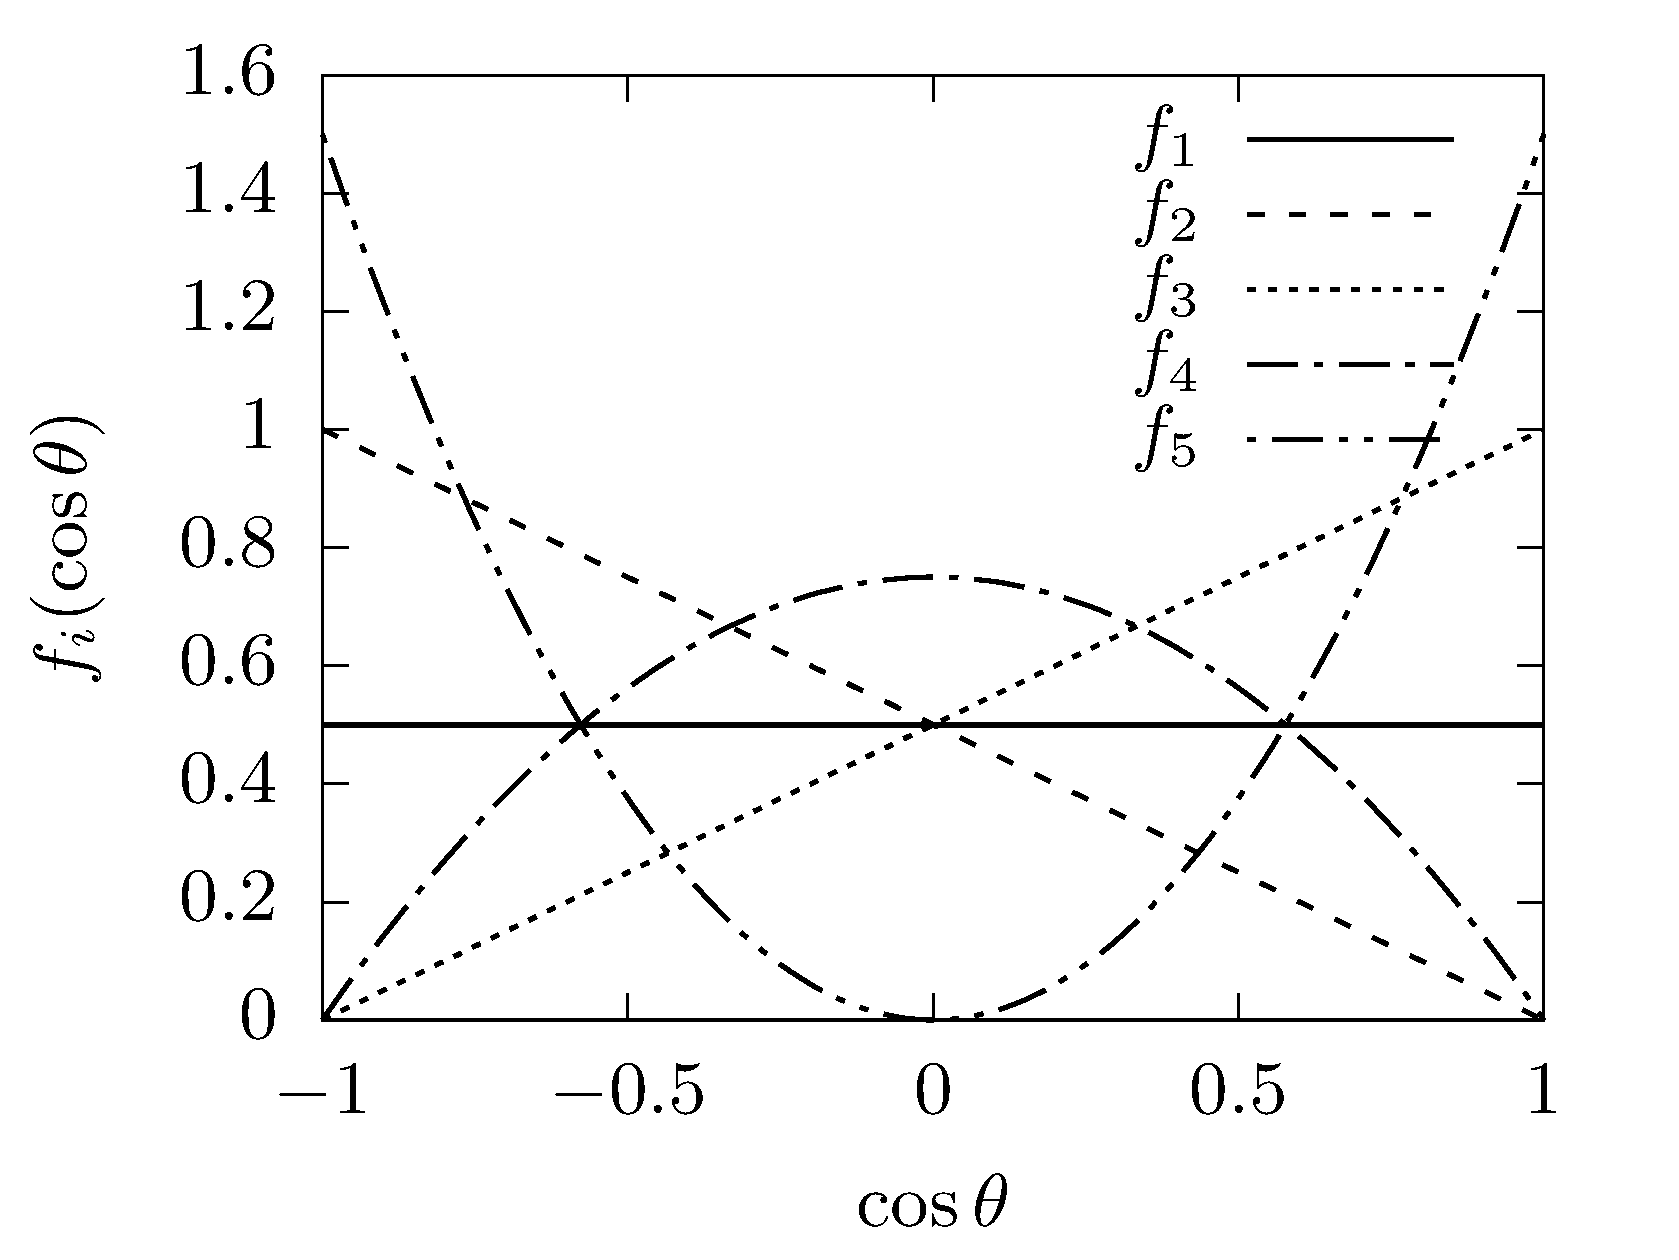
\includegraphics[scale=1.]{apdx_partbkg/f.png}
    \end{subfigure}
    \begin{subfigure}{.49\textwidth}
        \centering
        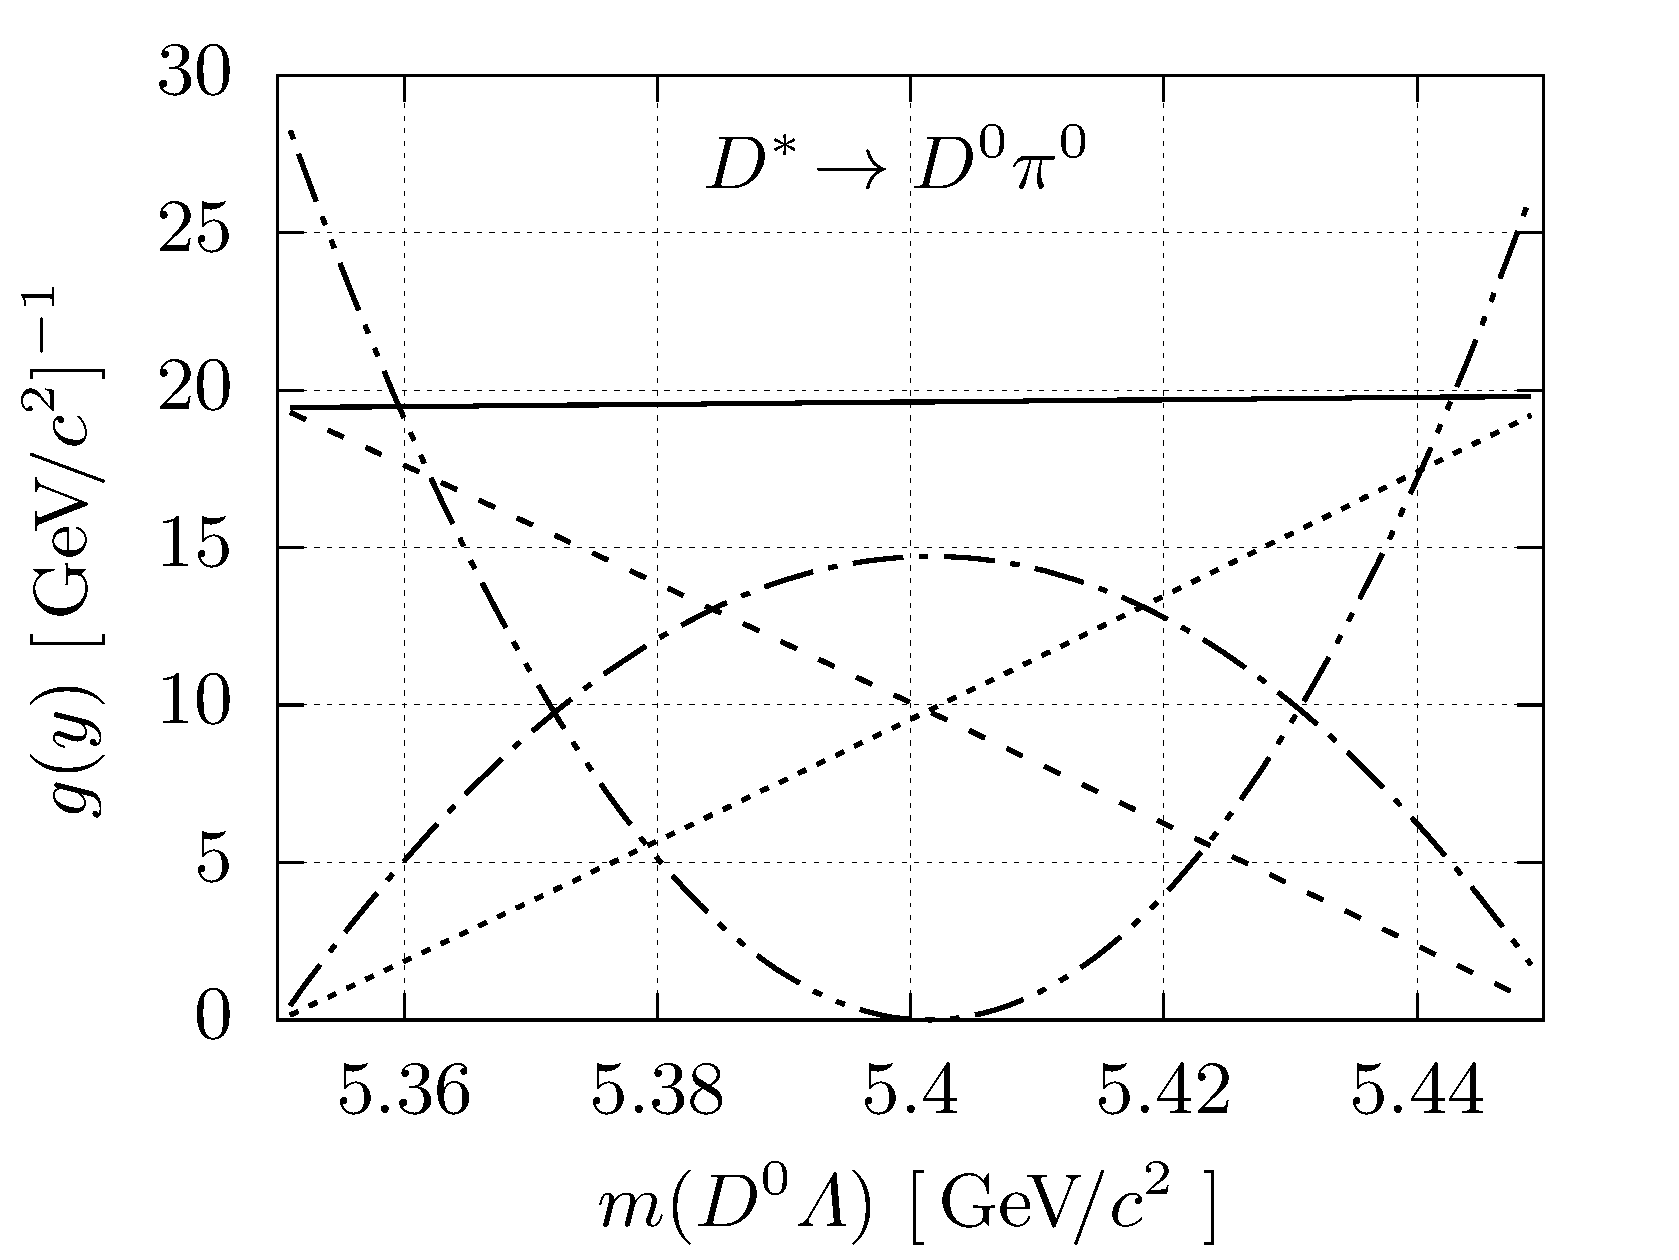
\includegraphics[scale=1.]{apdx_partbkg/gDzpiz.png}
    \end{subfigure}
    \caption{Distribution $g(m)$ for the decay \decay{\Lb}{\Dstarz\Lz} with \decay{\Dstarz}{\Dz\piz} (right) assuming different polarizations $f_i$ (left).}
    \label{fig:apdx_partbkg_pols}
\end{figure}
We note that the presence of polarization can change the shape significantly, \eg{}, $f_4$ suppresses $g(m)$ up to zero, whereas the enhancement of $f_5$ is maximal at the same point.
Furthermore, we note that the shape of $g(m)$ is also imposed by the values of $a$ and $b$ which makes the unpolarized shape of $g(m)$ very flat, whereas in three-body decays, such as $\decay{\Lb}{\Sz\Ph\Ph'}$, $g(m)$ by itself, is already steep~\cite{LbToLzhh}.
Another example for the implication of polarization is the decay of the pseudo-scalar particle \Bd into two vector particles, \decay{\Bd}{\PD\Kstarz}, where the very same partially reconstructed background \decay{\Dstarz}{\Dz\piz} and \decay{\Dstarz}{\Dz\Pgamma} had to be described and found to differ significantly from being unpolarized in both cases~\cite{BdToDzKstar}.

In recorded data this shape will typically be smeared out due to various factors, such as the limited resolution of the experimental setup.
A first order approximation is motivated by the central limit theorem and state that the smearing can be parametrized by a convolution with a centered Gaussian function $\mathcal{G}_c \equiv \mathcal{G}(x|\mu=0,\sigma)$.
For simple functions such as the partial quadratic polynomial $\mathcal{K}$,
\begin{equation*}
    \mathcal{K}(x|a,b) = \begin{cases}
        1 + ax + bx^2 &\text{for } x_1 < x < x_2 \,, \\
        0 & \text{else},
    \end{cases}
\end{equation*}
the convolution can be evaluated analytically:
\begin{equation}
    \label{eq:apdx_partbkg_kconvl}
    (\mathcal{K} * \mathcal{G}_c)(x) = \left. -\frac{1 + ax + b \left( \sigma^2 + x^2 \right)}{2} \operatorname{erf} \left( \frac{x-y}{\sqrt{2} \sigma} \right) - \sigma^2 \left(a + b(x + y) \right) \mathcal{G}(x|y, \sigma) \right|_{y=x_1}^{y=x_2},
\end{equation}
with
\begin{equation*}
    \mathcal{G}(x|\mu,\sigma) = \frac{1}{\sqrt{2 \pi \sigma^2}} \exp \left( -\frac{1}{2} \left( \frac{x-y}{\sigma} \right)^2 \right).
\end{equation*}
The normalization of $(\mathcal{K} * \mathcal{G}_c)(x)$ can also be found analytically by integration:
\begin{multline*}
    \int \!\mathrm{d}x \, (\mathcal{K} * \mathcal{G})(x) = -\left[ \frac{x-y}{2} + a \frac{x^2 - y^2 - 3\sigma^2}{4} + b \frac{x^3 + 3\sigma^2 x - y^3}{6} \right] \operatorname{erf} \left( \frac{x - y}{\sqrt{2} \sigma} \right) \\
    \left.- \left[ 1 + a \frac{x + y}{2} + b \frac{2\sigma^2 + x^2 + xy + y^2}{3} \right] \sigma^2 \mathcal{G}(x|y, \sigma) \right|_{y=x_1}^{y=x_2}.
\end{multline*}
If instead of using one Gaussian, a weighted sum centered Gaussian shapes $\mathcal{G}_{c,i}$ with zero mean but different widths $\sigma_i$ is used for the smearing, Eq.~\eqref{eq:apdx_partbkg_kconvl} can be generalized due to distributivity and associativity with scalar multiplication of convolutions:
\begin{align*}
    (\mathcal{K} * \sum_i w_i \, \mathcal{G}_{c,i})(x) &= \sum_i w_i (\mathcal{K} * \mathcal{G}_{c,i})(x) \\
    &= \left. - \sum_i \frac{1 + ax + b \left( \sigma_i^2 + x^2 \right)}{2} w_i \operatorname{erf} \left( \frac{x-y}{\sqrt{2} \sigma_i} \right) \right|_{y=x_1}^{y=x_2}\\
    & \quad \left. - \sum_i \sigma_i^2 \left(a + b(x + y) \right) \, w_i \, \mathcal{G}(x|y, \sigma_i) \right|_{y=x_1}^{y=x_2}.
\end{align*}
